\chapter{Análise de Resultados} \label{ch:analise_resultados}

Este capítulo apresenta a análise dos resultados obtidos a partir do desenvolvimento da linguagem proposta, organizados com relação aos objetivos específicos estabelecidos na \autoref{sec:objetivos}. Após avaliar como cada objetivo específico foi alcançado, eles serão sintetizados para determinar se o objetivo geral do trabalho foi atingido.

\section{Implementação da Solução}

A implementação do protótipo de interpretador para a linguagem proposta se mostrou muito parecida com a implementação de interpretadores de linguagens tradicionais. Isso se deve ao fato dele possuir todas as fases genéricas de um interpretador tradicional implementadas, já que foi feito com base na primeira metade do livro \textit{Crafting Interpreters}, e consequentemente feito com base em Jlox \cite{craftinginterpreters}.

Saindo do escopo de fases de um interpretador e indo mais a fundo na implementação, também foi possível observar semelhanças de sintaxe com linguagens tradicionais. Um exemplo disso é a sintaxe de declaração de sistemas, que é muito parecida com a sintaxe de declaração de funções em Jlox, Rust, e muitas outras linguagens \cite{rustbook,craftinginterpreters}. A figura \ref{fig:decl_sistema_funcao} demonstra essa semelhança usando regras de produção.

\begin{figure}[H]
	\centering
	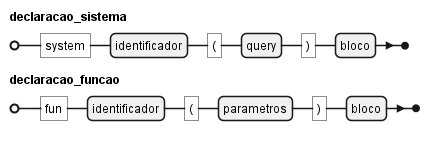
\includegraphics[width=0.45\textheight]{../diagrams/decl_sistema_funcao.png}
	\caption{Diagrama de sintaxe comparando declaração de sistemas e funções.}
	\fonte{Elaboração própria com PlantUML feita com base no interpretador nosso e no de Jlox \cite{craftinginterpreters}.}
	\label{fig:decl_sistema_funcao}
\end{figure}

Fora as semelhanças, as diferenças da linguagem proposta se encontram principalmente na semântica e pragmática, que foram adaptadas para suportar os conceitos de ECS.

\section{Decisões Tomadas e Desafios Encontrados}

\section{Viabilidade e Limitações da Solução}

\section{Síntese dos Resultados}
